\documentclass{article}
\usepackage{fancyhdr}
\usepackage{amsmath}
\usepackage{amsthm}
\usepackage{amssymb}
\usepackage{graphicx}
\usepackage{float}
\usepackage{subcaption}
\usepackage{hyperref}
\usepackage{listings}
\usepackage{color}
\usepackage{tikz}
\usepackage{soul}
\usepackage{pgfplots}
\usepackage{pgfplotstable}
\usepackage{listings}
\usepackage{color}
\usepackage{tikz}
\usepackage{amsthm}
\usepackage[margin=15mm]{geometry}

\definecolor{dkgreen}{rgb}{0,0.6,0}
\definecolor{gray}{rgb}{0.5,0.5,0.5}
\definecolor{mauve}{rgb}{0.58,0,0.82}

% Set up fancy header
\pagestyle{fancy}
\fancyhf{} % Clear default header and footer
\rhead{Keith Wesa} % Right header
\lhead{CS 151 1.10 Notes:} % Left header
\rfoot{Page \thepage} % Right footer

\author{Keith Wesa}
\title{MAT 215 - Written Homework 1}
\date{\today}

\begin{document}
\section*{1.10 Nested Quantifiers}
\subsection*{More Nested Quantified Statements}
\begin{itemize}
    \item[] \textbf{Using logic to express "everyone else"}
    \item Consider a scenario where the domain is a group of people who are all working on a joint project. Let $M(x,y)$ be the predicate
    ``$x$ has sent an e-mail message to $y$''. The statement $\forall x \forall y M(x,y)$ asserts that everyone has sent an e-mail message to themselves
    How can we use logic to express that everyone sent an e-mail to everyone without sending it to themselves? The idea is to use a conditional operation:
    \item[] $(x \neq y) \rightarrow M(x,y)$
    \begin{center}
        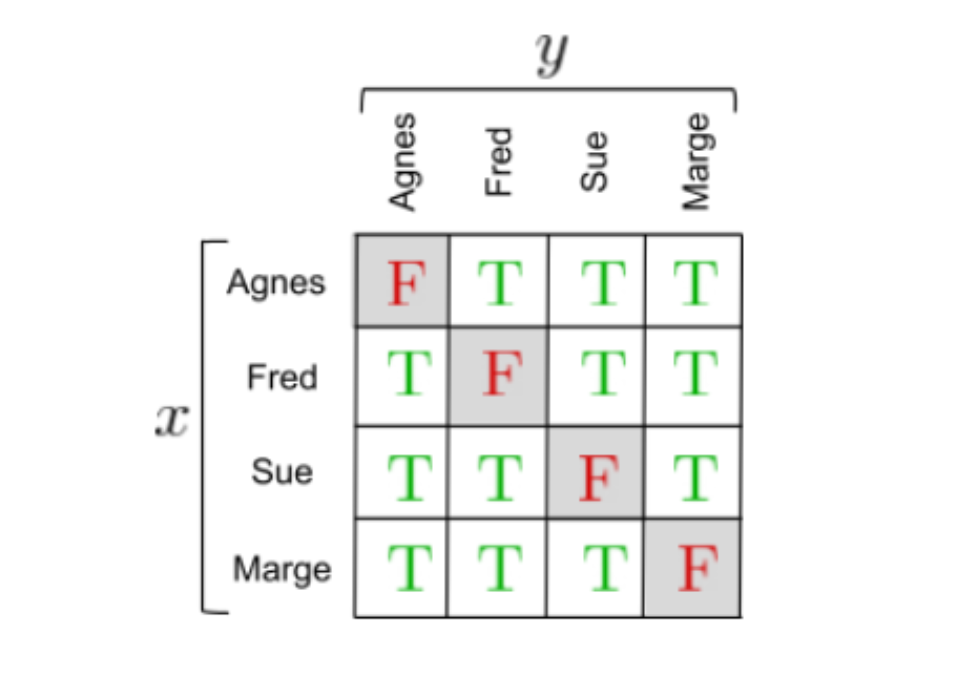
\includegraphics[scale=0.5]{1.10_TruthTable_1.png}
    \end{center}
    \item The statement $\forall x \forall y M(x,y)$ is false because M(Fred, Fred) and M(Marge, Marge) are both false
    \item The statement $\forall x \forall y ((x \neq y) \rightarrow M(x,y))$ is true because the only false case is when $x = y$ and $M(x,y)$ is false
\end{itemize}
\subsection*{Expressing uniqueness in quantified statements}
An existentially quantified statement evaluates to true even if there is more than one element in the domain that causes the predicate tot evaluate to true. 
If the domain is a set of people who attended a meeting and the predicate $L(x)$ indicates whether or not $x$ came late to the meeting, the statement $\exists x L(x)$
is true if there are on or more people who came late.

\end{document}  